\documentclass[10pt]{article}
% Shared preamble for model_card.tex and assumptions_register.tex
\usepackage[T1]{fontenc}
\usepackage[utf8]{inputenc}
\usepackage{lmodern}
\usepackage[margin=2cm]{geometry}
\usepackage{amsmath,amssymb}
\usepackage{graphicx}
\usepackage{booktabs,longtable,tabularx,array,multirow}
\usepackage[table]{xcolor}
\usepackage{enumitem}
\usepackage{caption}
\usepackage[hidelinks]{hyperref}
\usepackage{xurl}
\usepackage{pdflscape}

\graphicspath{{figures/}}
\setlist{itemsep=2pt,topsep=3pt}
\captionsetup{font=small,labelfont=bf}
\renewcommand{\arraystretch}{1.15}

% ---- editing helpers -------------------------------------------------------
% \TODO{...} marks text the students still have to write or confirm (renders red in the PDF).
\newcommand{\TODO}[1]{\textcolor{red!75!black}{\textbf{[TODO:} #1\textbf{]}}}
% Single source for facts that appear in both documents; edit here, not in the text.
\newcommand{\Nall}{138{,}554}
\newcommand{\Nhh}{85{,}182}
\newcommand{\prev}{0.631}
\newcommand{\capacity}{30\%}
\newcommand{\epsTol}{0.10}
\newcommand{\minSupport}{30}
\newcommand{\nbDate}{25 October 2026}
% Team facts used by every document in writeup/, report/ and slides/. Edit here once.
\newcommand{\StudentA}{Sumedh Navuda}
\newcommand{\StudentB}{Aldino}
\newcommand{\Authors}{\StudentA{} and \StudentB{}}
\newcommand{\Contact}{sumedhnavuda@outlook.com}
\newcommand{\RollA}{[roll no.]}   % <- replace with Sumedh's roll number
\newcommand{\RollB}{[roll no.]}   % <- replace with Aldino's roll number
\newcommand{\RepoURL}{https://github.com/sumedhnvda/ict5143-p8-fairness-audits}
\newcommand{\TeamID}{[team ID]}   % <- replace with the team ID given by the instructor
\newcommand{\SubmitTag}{submission-v1}
   % names, roll numbers, contact, repository (shared with report/ and slides/)
\newcommand{\nb}{\texttt{Problem8\_\allowbreak Intersectional\_\allowbreak Fairness.ipynb}}
\newcommand{\sect}[1]{notebook~\S#1}
\newcommand{\status}[1]{\textsf{\small #1}}


\title{Model Card\\[2pt]\large Bayesian-network outreach ranking and Bayesian intersectional audit\\
ACSPublicCoverage, California 2018 (ICT 5143 Capstone, Problem 8)}
\author{\Authors\\ \small Contact: \texttt{\Contact}}
\date{Version 1.0 \textperiodcentered{} results from the executed notebook of \nbDate}

\begin{document}
\maketitle

\noindent\fbox{\parbox{\dimexpr\textwidth-2\fboxsep}{\small
\textbf{Read first.} $Y=1$ means \emph{no public health coverage} in the ACS person record. It does \textbf{not} mean
uninsured and it does \textbf{not} mean eligible for any programme. $D=1$ means selection for \emph{hypothetical}
information outreach. This model is a research artefact for studying fairness audits. It must not be used to make or
support decisions about real people. All numbers come from \nb{} with fixed seeds. Synthetic and semi-synthetic results
describe the procedures, not the California population.}}

\section{Model details}
\begin{itemize}
  \item \textbf{Developers:} \Authors, ICT 5143 Algorithms, Fairness and Graphical Models Laboratory. Contact: \texttt{\Contact}. Repository: \url{\RepoURL}.
  \item \textbf{Date and version:} v1.0, \nbDate. Code: \nb{} (self-contained, executed); environment pinned in \texttt{requirements-\allowbreak lock.txt}.
  \item \textbf{Predictive model:} a discrete Bayesian network with an augmented naive-Bayes structure (Figure~\ref{fig:bn}).
    $Y$ is a parent of all 18 features, plus the feature edges SCHL$\mid$AGEP, ESR$\mid$AGEP, PINCP$\mid$ESR,
    DIS$\mid$AGEP, MAR$\mid$AGEP, CIT$\mid$NATIVITY, \{DEAR, DEYE, DREM\}$\mid$DIS and FER$\mid$SEX. ST is constant
    within one state and is omitted. The CPTs are Dirichlet-smoothed ($\alpha=1$), which makes every entry positive.
    AGEP and SCHL use fixed bins, and PINCP uses training-split quartiles. \textbf{The graph is associational, not causal.}
  \item \textbf{Inference:} exact. $P(Y\mid\text{evidence})$ by variable elimination. Our VE under two elimination orders,
    pgmpy VE, pgmpy clique-tree belief propagation and enumeration agree to $3.3\times10^{-16}$ over 200 random evidence
    masks. The vectorised predictor equals general VE, and the joint CI $\text{SEX}\perp\{\text{AGEP},\text{DIS}\}\mid Y$
    holds in the fitted model (\sect{3.1}).
  \item \textbf{Decision rule:} $D=1$ if the predicted probability is in the top \capacity{} of validation scores
    (group-unaware, $\lambda=0$). Fairness-adjusted variants $R(\lambda)$ blend the global threshold with group-specific
    equal-opportunity thresholds: $t_g(\lambda)=(1-\lambda)t_{\text{global}}+\lambda t_g^{\text{EOpp}}+c$, with $c$ set
    so that exactly \capacity{} of validation records are selected. $\lambda$ is chosen on validation only (\sect{10}).
  \item \textbf{Baselines:} logistic regression (one-hot categories plus scaled AGEP, SCHL, PINCP) and histogram
    gradient-boosted trees (300 iterations, learning rate 0.08), with the same information and splits.
  \item \textbf{Audit models} (for $k_g\sim\text{Bin}(n_g,\theta_g)$, where $n_g$ = positives and $k_g$ = selected positives in
    intersection $g$): raw $k/n$; independent Beta(1,1); complete pooling; empirical-Bayes beta-binomial (hier); full-Bayes
    beta-binomial on a grid; the attribute-structured hierarchical logistic audit (struct), with
    $\operatorname{logit}\theta_g=\beta_0+\beta_{\text{race}}+\beta_{\text{sex}}+\beta_{\text{dis}}+u_g$ and
    $u_g\sim N(0,\tau^2)$; and the \textbf{proposed} $\epsilon$-contamination prior
    $\theta_g\sim\pi\,\text{Beta}(a,b)+(1-\pi)\,\text{Beta}(1,1)$ with $\pi\le\pi_{\max}$ (Figure~\ref{fig:audit}).
    The struct model is a documented restricted version of a hierarchical intersectional audit in the spirit of Foulds et al.
    It is \emph{not} an exact reproduction of their model.
  \item \textbf{Calibrated audit procedure (frozen in \sect{9}):} contamination prior with $\pi_{\max}=0.8$ and the
    plug-in rule ``declare $\Delta\text{EOpp}\le\epsilon$ if the max$-$min of the posterior mean TPRs is $\le\epsilon$''.
    It was chosen by a preregistered Youden criterion on synthetic data before any real-data selection.
  \item \textbf{Recommended procedure (\sect{15}):} \emph{design-matched calibration} of the contamination audit (slab type,
    $\pi_{\max}$ and rule chosen by the same Youden criterion on semi-synthetic worlds built from the deployment population's
    validation group sizes), plus \emph{held-out certification} (choose $\lambda$ on half of the validation households,
    certify on the other half). Chosen configurations: CA, fixed slab with $\pi_{\max}=0.99$ and the upper-0.9 rule; TX,
    centred slab with $\pi_{\max}=0.95$ and the upper-0.5 rule.
  \item \textbf{Licence:} MIT licence for our code (\texttt{LICENSE}). The data are public-domain ACS PUMS and are not redistributed.
  \item \textbf{Citation:} S.~Navuda and Aldino. \emph{When does pooling make intersectional fairness audits falsely reassuring?} ICT 5143 capstone report, Problem 8, 2026. \url{\RepoURL}.
\end{itemize}

\begin{figure}[h]
  \centering
  \begin{minipage}{0.52\textwidth}\centering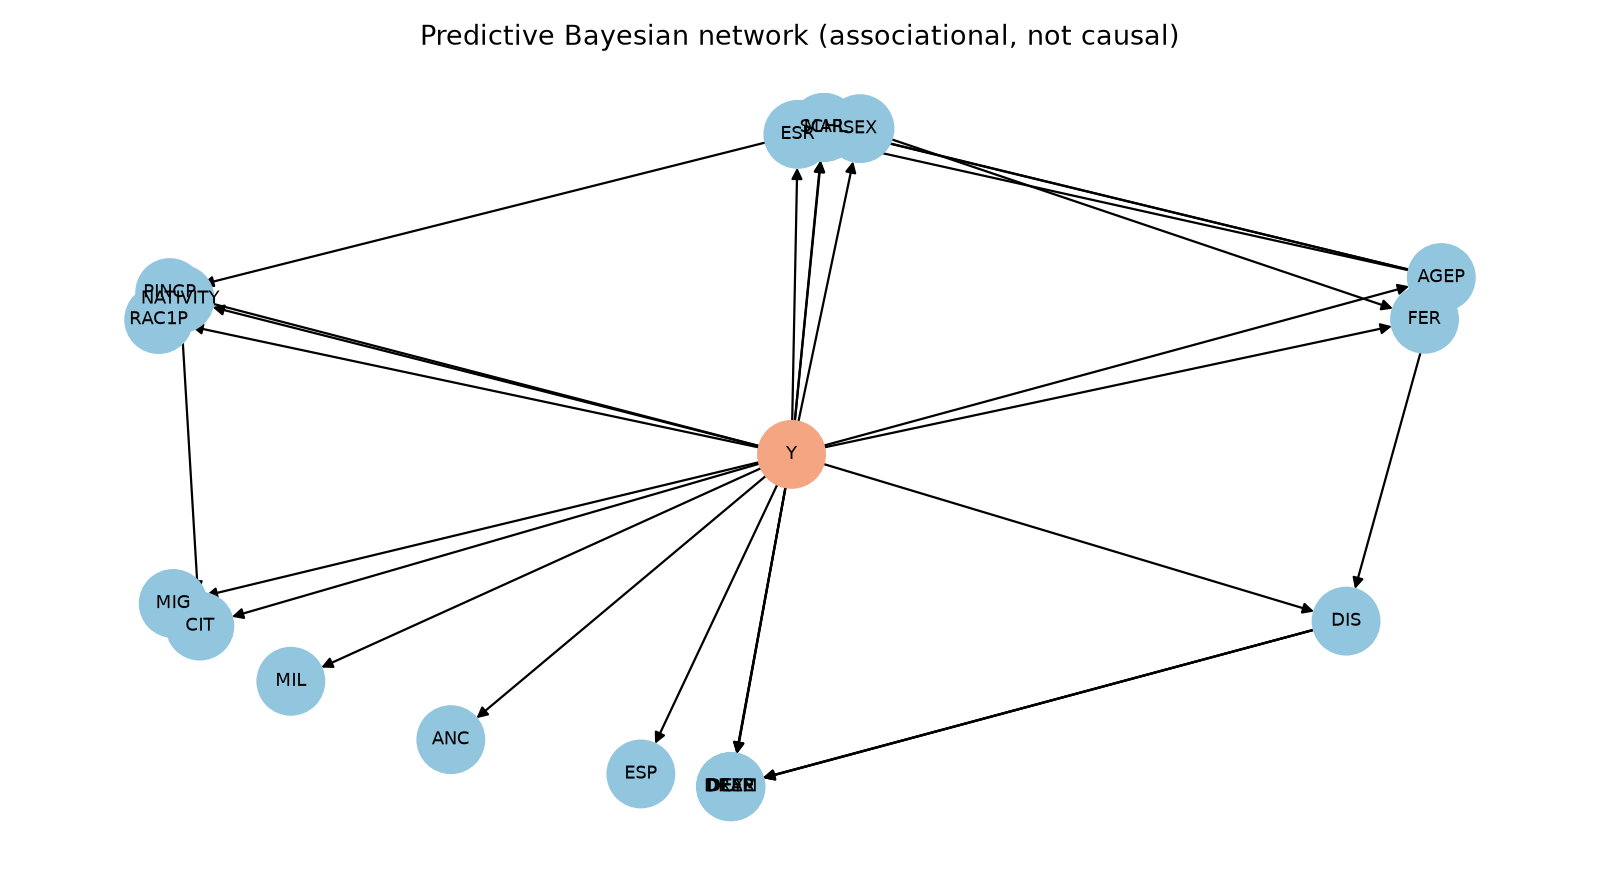
\includegraphics[width=\linewidth]{bn_structure.png}
    \caption{Predictive BN structure (associational).}\label{fig:bn}\end{minipage}\hfill
  \begin{minipage}{0.45\textwidth}\centering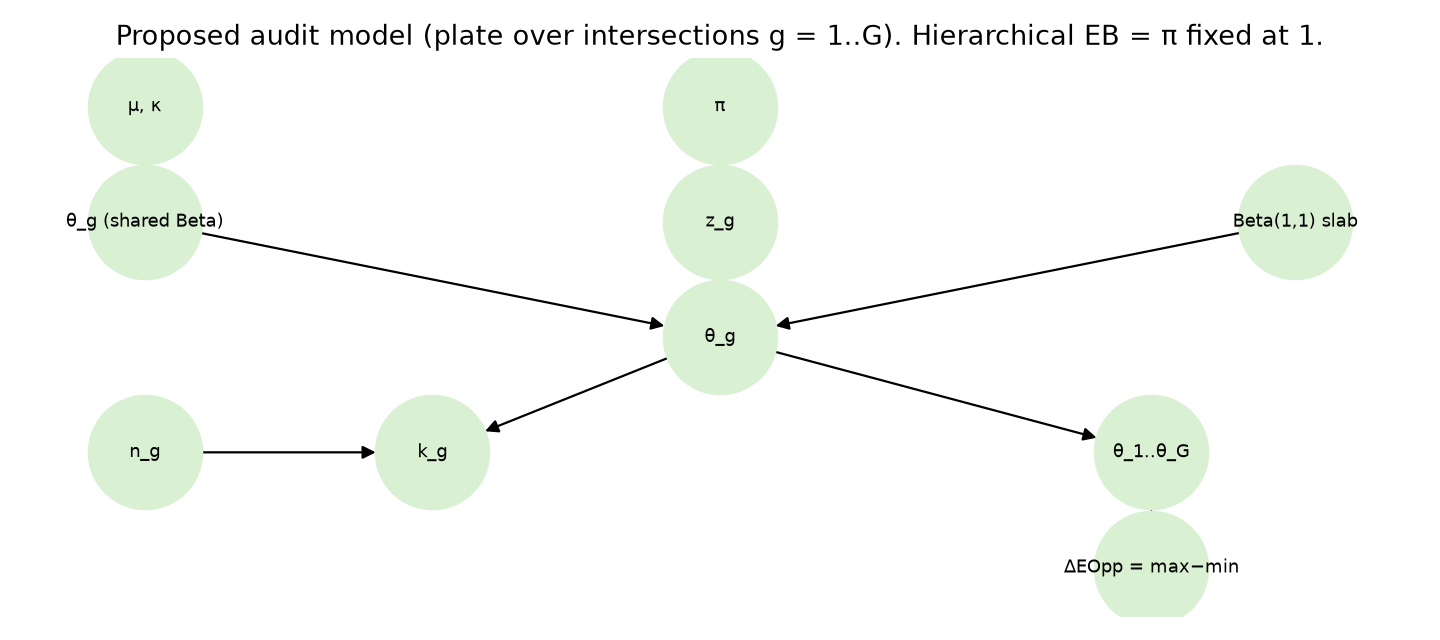
\includegraphics[width=\linewidth]{audit_model_structure.png}
    \caption{Proposed audit model (plate over intersections). Hierarchical EB is the case $\pi=1$.}\label{fig:audit}\end{minipage}
\end{figure}

\section{Intended use}
\begin{itemize}
  \item \textbf{Primary use:} a benchmark for studying when Bayesian intersectional fairness audits are reliable, in
    particular whether partial pooling hides a small disadvantaged intersection and whether validation-time tolerance
    claims hold on independent data.
  \item \textbf{Primary users:} fairness auditors, researchers and course staff. The stakeholders named in the problem are
    low-income residents, public-health outreach teams and community organisations.
  \item \textbf{Out of scope:} deciding who is contacted, enrolled or denied anything; inferring a person's insurance status or
    programme eligibility; any causal statement about race, sex or disability; use for another state, year or population
    without re-validation and re-calibration (\S\ref{sec:caveats}); certifying that a rule is ``fair''.
\end{itemize}

\section{Factors}
\begin{itemize}
  \item \textbf{Protected attributes as recorded:} RAC1P (nine source codes, not collapsed), SEX (1 male, 2 female) and
    DIS (1 with a disability, 2 without). These are self- or proxy-reported survey categories and limited measurements of
    identity. Nothing is inferred from names or other variables.
  \item \textbf{Intersections:} race $\times$ sex $\times$ disability gives 36 cells, of which 35 are non-empty in the seed-0 test
    split. Two-attribute groupings (race$\times$sex, sex$\times$disability, race$\times$disability) and single attributes
    are reported as baselines.
  \item \textbf{Small groups:} cells with fewer than \minSupport{} positives or negatives are flagged exploratory and
    reported, never dropped. In the seed-0 test split, 14 of the 35 non-empty intersections have fewer than 30 positives,
    and one (\texttt{7|2|1}) has none.
  \item \textbf{Use of protected attributes at prediction time:} all three models use RAC1P, SEX and DIS as features, as in
    the Folktables definition. Rules with $\lambda>0$ also use group-specific thresholds.
\end{itemize}

\section{Metrics}
\begin{itemize}
  \item \textbf{Primary predictive metric:} recall at \capacity{} outreach capacity. Also AUROC, average precision,
    precision at capacity, log loss, Brier score, per-group expected calibration error and worst-group recall.
  \item \textbf{Primary fairness metric:} intersectional equality of opportunity,
    $\Delta\text{EOpp}=\max_g t_g-\min_g t_g$ over intersections with $\ge\minSupport$ positives, with tolerance
    $\epsilon=\epsTol$ (robustness: 0.05, 0.15). The diagnostics are $\Delta$DP, $\Delta$EOdds, the selection-rate
    ratio $R_{\text{sel}}$ and the worst-group TPR.
  \item \textbf{Model-based audit metrics:} posterior intervals for $\Delta$EOpp, $P(\Delta\text{EOpp}>\epsilon\mid\text{data})$,
    and in simulation the false tolerance-satisfaction rate (FTS = $P$(declared fair $\mid$ truly unfair)), the correct
    acceptance rate (ACC = $P$(declared fair $\mid$ truly fair)), interval coverage and width.
  \item \textbf{Uncertainty:} \emph{evaluation} uncertainty from 1,000 household-cluster (Poisson) bootstrap replicates of
    the seed-0 test split; \emph{training} uncertainty from 5 refits on independent household splits. They are reported separately.
  \item \textbf{Acceptable utility loss (preregistered):} at most 0.02 recall relative to the unconstrained rule.
\end{itemize}

\section{Training and evaluation data}
\begin{itemize}
  \item \textbf{Source:} US Census Bureau, American Community Survey PUMS 2018 1-Year person file for California, obtained through
    \texttt{folktables.ACSDataSource(...).get\_data(download=True)}.
  \item \textbf{Task definition:} Folktables \texttt{ACSPublicCoverage} (\texttt{public\_coverage\_filter}: AGEP $<65$ and
    PINCP $\le30{,}000$), giving \Nall{} people in \Nhh{} households. Our features are identical, cell by cell, to
    Folktables' \texttt{df\_to\_numpy} output. Label $Y=1-\mathbb 1[\text{PUBCOV}=1]$ (exact reversal), with prevalence \prev{}.
  \item \textbf{Splits:} household-disjoint 60/20/20 (train/validation/test) on SERIALNO, five split seeds. Bins, CPTs,
    thresholds, $\lambda$ and audit hyperparameters use training and validation data only. The test split is used only to
    audit frozen rules.
  \item \textbf{Bookkeeping columns, not features:} SERIALNO (splits and clustered bootstrap); PWGTP and PWGTP1--80
    (survey-weighted estimates, \sect{13}).
  \item \textbf{Replication population:} Texas 2018 (98,928 people), with identical definitions (\sect{14}).
\end{itemize}

\section{Quantitative analyses}
\subsection{Predictive performance and unconstrained-rule fairness}
\begin{table}[h]\centering\small
\caption{Test metrics of the unconstrained top-\capacity{} rule, mean $\pm$ sd over 5 household splits.}\label{tab:pred}
% generated by make_tables.py from ../results; do not edit by hand
\begin{tabular}{lccc}
\toprule
Metric & BN & LR & GBT \\
\midrule
AUROC & 0.729 $\pm$ 0.004 & 0.716 $\pm$ 0.004 & 0.768 $\pm$ 0.003 \\
AP & 0.803 $\pm$ 0.002 & 0.787 $\pm$ 0.002 & 0.836 $\pm$ 0.002 \\
Recall@30\% & 0.388 $\pm$ 0.005 & 0.384 $\pm$ 0.006 & 0.409 $\pm$ 0.006 \\
Prec.@30\% & 0.824 $\pm$ 0.004 & 0.809 $\pm$ 0.004 & 0.860 $\pm$ 0.002 \\
Log loss & 0.577 $\pm$ 0.004 & 0.584 $\pm$ 0.002 & 0.541 $\pm$ 0.003 \\
Brier & 0.196 $\pm$ 0.002 & 0.199 $\pm$ 0.001 & 0.182 $\pm$ 0.001 \\
max group ECE & 0.110 $\pm$ 0.010 & 0.069 $\pm$ 0.011 & 0.063 $\pm$ 0.013 \\
$\Delta$EOpp & 0.719 $\pm$ 0.018 & 0.625 $\pm$ 0.049 & 0.585 $\pm$ 0.019 \\
$\Delta$DP & 0.655 $\pm$ 0.016 & 0.548 $\pm$ 0.021 & 0.508 $\pm$ 0.013 \\
worst recall & 0.000 $\pm$ 0.000 & 0.000 $\pm$ 0.000 & 0.008 $\pm$ 0.011 \\
\bottomrule
\end{tabular}

\end{table}

The BN is roughly at the level of logistic regression (AUROC 0.729 vs 0.716). Gradient-boosted trees are best (0.768).
Predictive accuracy is not the contribution. The BN's worst per-group calibration error (0.110) is larger than LR's
(0.069) and GBT's (0.063); see Figure~\ref{fig:calib}.

\subsection{Single-attribute vs intersectional audit}
\begin{table}[h]\centering\small
\caption{Seed-0 test split, unconstrained rule. Gaps use groups with $\ge$30 relevant observations (adequate/all).}\label{tab:exp1}
\resizebox{\textwidth}{!}{% generated by make_tables.py from ../results; do not edit by hand
\begin{tabular}{lc*{9}{c}}
\toprule
& & \multicolumn{3}{c}{BN} & \multicolumn{3}{c}{LR} & \multicolumn{3}{c}{GBT} \\
\cmidrule(lr){3-5}\cmidrule(lr){6-8}\cmidrule(lr){9-11}
Grouping & adequate/all & $\Delta$EOpp & $\Delta$DP & worst rec. & $\Delta$EOpp & $\Delta$DP & worst rec. & $\Delta$EOpp & $\Delta$DP & worst rec. \\
\midrule
SEX & 2/2 & 0.162 & 0.128 & 0.291 & 0.080 & 0.060 & 0.338 & 0.095 & 0.077 & 0.346 \\
DIS & 2/2 & 0.384 & 0.324 & 0.021 & 0.396 & 0.334 & 0.010 & 0.354 & 0.307 & 0.067 \\
RACE & 8/9 & 0.597 & 0.548 & 0.079 & 0.561 & 0.456 & 0.106 & 0.360 & 0.313 & 0.169 \\
SEX$\times$DIS & 4/4 & 0.468 & 0.386 & 0.009 & 0.436 & 0.361 & 0.004 & 0.427 & 0.352 & 0.034 \\
RACE$\times$SEX & 14/18 & 0.678 & 0.614 & 0.059 & 0.611 & 0.517 & 0.099 & 0.429 & 0.410 & 0.155 \\
RACE$\times$DIS & 13/18 & 0.697 & 0.634 & 0.000 & 0.686 & 0.554 & 0.000 & 0.544 & 0.464 & 0.000 \\
RACE$\times$SEX$\times$DIS & 21/35 & 0.746 & 0.683 & 0.000 & 0.711 & 0.580 & 0.000 & 0.600 & 0.519 & 0.000 \\
\bottomrule
\end{tabular}
}
\end{table}

\textbf{Aggregate audits hide most of the disparity.} For the BN, $\Delta$EOpp is 0.162 by sex and 0.384 by disability,
0.468 for sex$\times$disability, and \textbf{0.746 intersectionally}. Every disabled intersection has a TPR of at most
0.08. Disabled low-income adults mostly \emph{do} have public coverage, so the model ranks them low, and the minority of
them without coverage would almost never be reached. Survey weighting does not change this. The weighted test TPR is
0.011 (SE 0.006) for disabled men and 0.031 (0.009) for disabled women, against 0.280 (0.006) and 0.448 (0.006) for men and
women without a disability (80 successive-difference replicate weights). Texas 2018 replicates the pattern: 0.094 by sex,
0.390 by disability, 0.432 for sex$\times$disability, 0.888 intersectionally.

\begin{figure}[h]\centering
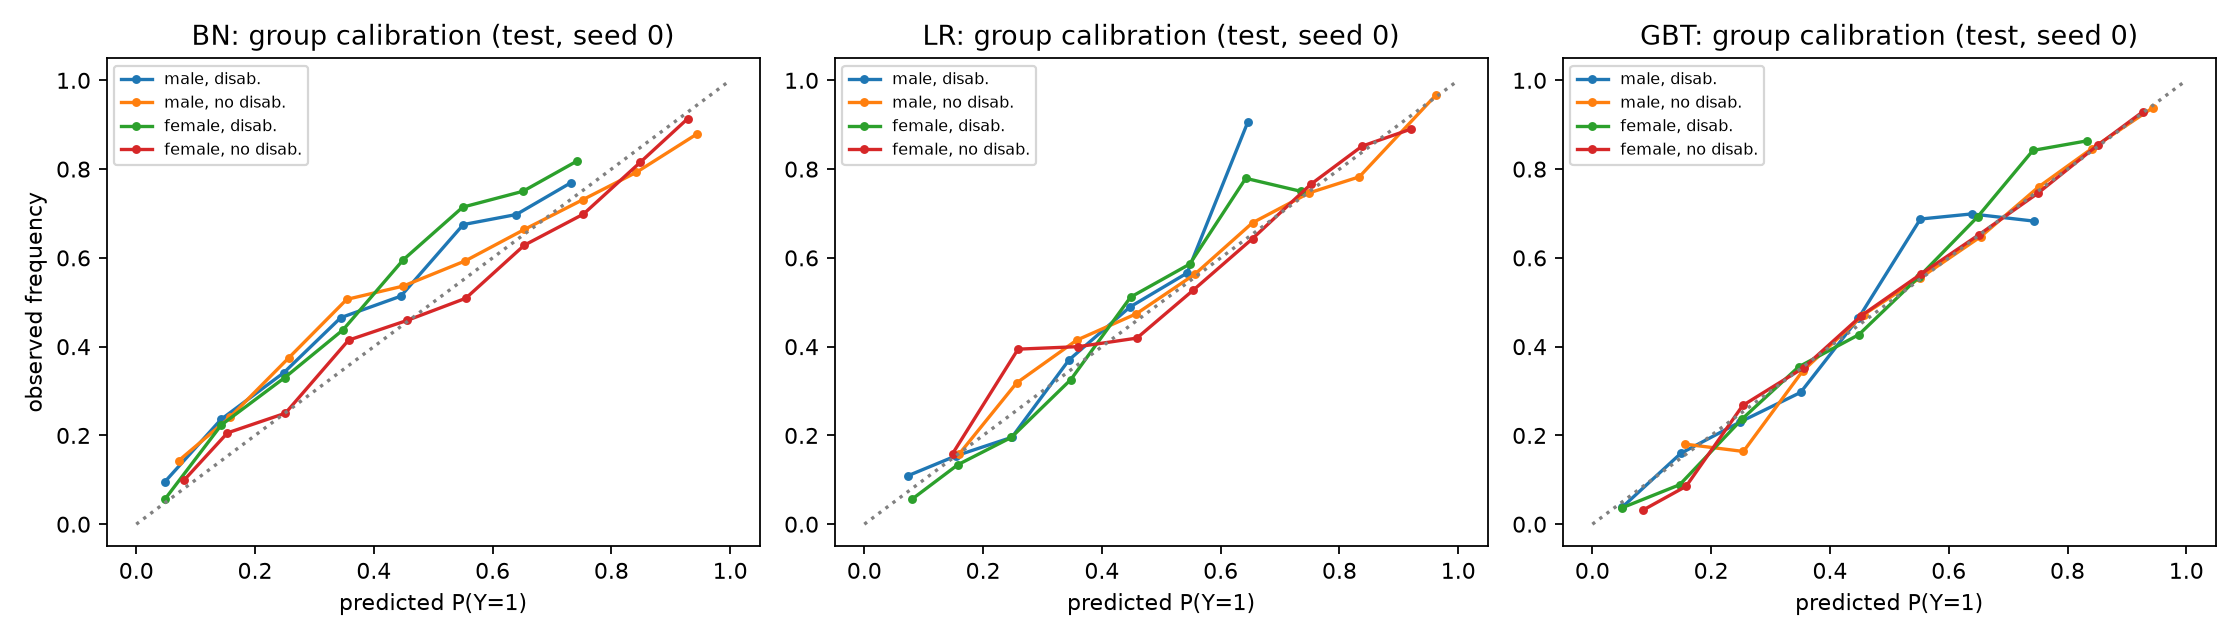
\includegraphics[width=\textwidth]{group_calibration.png}
\caption{Group calibration by sex$\times$disability (test, seed 0).}\label{fig:calib}
\end{figure}

\subsection{Audit-model behaviour on real counts}
Table~\ref{tab:groups} (appendix) lists every intersection with its denominators. Pooling moves estimates appreciably only
for groups with 1--7 positives (pull 0.05--0.14), and no group with $\ge$30 positives moves by more than 0.032
(Figure~\ref{fig:pull}). On these counts the struct model fits $\hat\tau=0.01$ (its lower bound) and reduces to a
main-effects logistic model. It gives an implausibly narrow 90\% interval for $\Delta$EOpp, (0.750, 0.757), against
(0.729, 0.816) for hier. Every audit model gives $P(\Delta\text{EOpp}>0.10\mid\text{data})=1.0$ for the unconstrained rule,
at every tolerance and prior tested (\sect{12}).

\begin{figure}[h]\centering
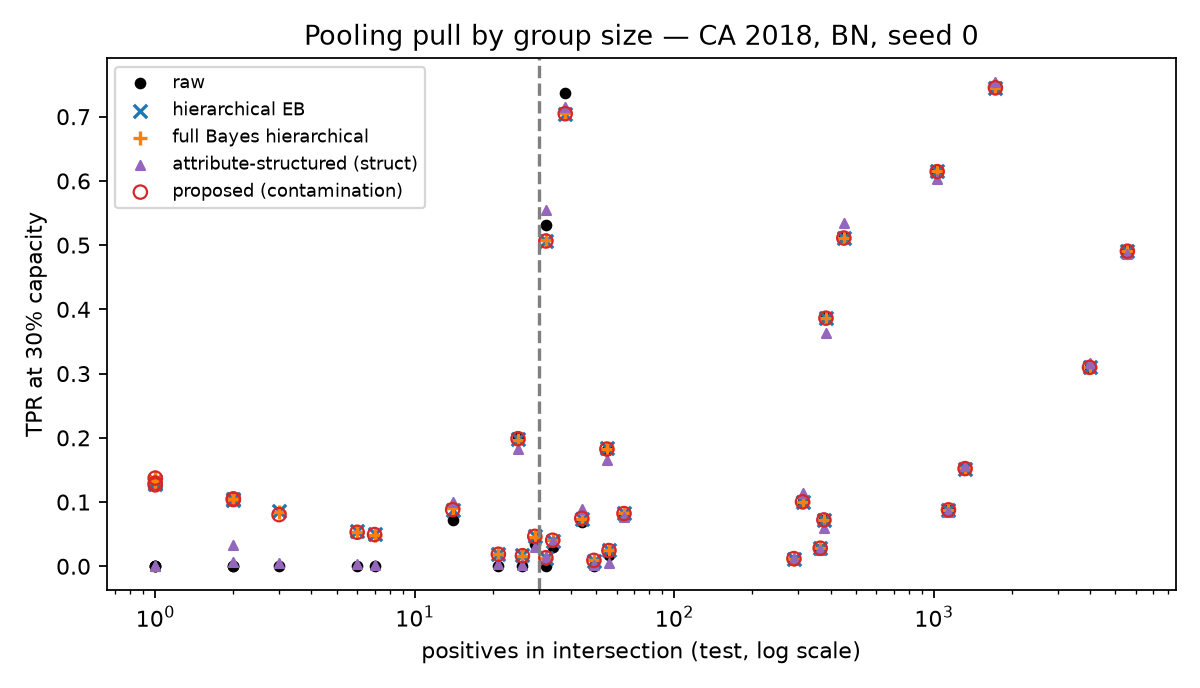
\includegraphics[width=0.72\textwidth]{real_pooling_pull.png}
\caption{Raw and pooled TPR estimates by intersection size (BN, seed 0, test).}\label{fig:pull}
\end{figure}

\subsection{Fairness-adjusted rules selected on validation}
\begin{table}[h]\centering\small
\caption{Intact training data, 5 household splits. ``Feasible'' = the criterion found a $\lambda$ with value $\le\epsilon$ on
validation. The test $P(\Delta>\epsilon)$ comes from the calibrated contamination audit on test counts.}\label{tab:sel}
\resizebox{\textwidth}{!}{% generated by make_tables.py from ../results; do not edit by hand
\begin{tabular}{lcccccccc}
\toprule
Selection criterion & feasible on val. & mean $\lambda$ & test recall & test sel. rate & test $\Delta$EOpp (mean $\pm$ sd) & worst recall & test $P(\Delta>\epsilon)$ \\
\midrule
raw $\cdot$ plug-in & 0/5 & 0.80 & 0.385 & 0.299 & 0.348 $\pm$ 0.077 & 0.172 & 0.997 \\
independent $\cdot$ upper & 0/5 & 0.84 & 0.383 & 0.299 & 0.418 $\pm$ 0.094 & 0.191 & 0.996 \\
complete $\cdot$ plug-in & 5/5 & 0.26 & 0.390 & 0.298 & 0.641 $\pm$ 0.066 & 0.019 & 1.000 \\
hier EB $\cdot$ plug-in & 5/5 & 0.90 & 0.383 & 0.299 & 0.323 $\pm$ 0.077 & 0.210 & 0.965 \\
hier EB $\cdot$ upper & 5/5 & 1.00 & 0.380 & 0.299 & 0.367 $\pm$ 0.060 & 0.260 & 0.952 \\
full Bayes $\cdot$ upper & 5/5 & 1.00 & 0.380 & 0.299 & 0.367 $\pm$ 0.060 & 0.260 & 0.950 \\
struct $\cdot$ plug-in & 2/5 & 1.00 & 0.380 & 0.299 & 0.367 $\pm$ 0.060 & 0.260 & 0.955 \\
struct $\cdot$ upper & 2/5 & 1.00 & 0.380 & 0.299 & 0.367 $\pm$ 0.060 & 0.260 & 0.950 \\
\textbf{proposed $\cdot$ plug-in (calibrated)} & 5/5 & 0.96 & 0.381 & 0.299 & 0.332 $\pm$ 0.072 & 0.245 & 0.921 \\
proposed $\cdot$ upper & 0/5 & 1.00 & 0.380 & 0.299 & 0.367 $\pm$ 0.060 & 0.260 & 0.952 \\
\bottomrule
\end{tabular}
}
\end{table}

\textbf{Every validation-time ``tolerance satisfied'' claim was false on test.} The pooled criteria (hier, full Bayes,
complete pooling, the calibrated proposed rule, and struct in 2 of 5 splits) found a $\lambda$ meeting $\epsilon=0.10$ on
validation. Across all splits and thinning levels, all 116 such claims had a test $\Delta$EOpp between 0.227 and 0.770.
Raw and independent criteria never made the claim. The utility cost of the most fairness-seeking rule ($\lambda=1$) is
0.008 recall on average (at most 0.013 in any split), within the 0.02 budget. Figure~\ref{fig:tradeoff} shows the
trade-off curves. In the confirmatory tests, the calibrated rule and hier plug-in chose the same $\lambda$ at seed 0
($\Delta=0$). Against raw plug-in the difference is $-0.052$, 95\% CI $[-0.194, 0.051]$, Holm $p=0.736$.
Across the 5 refits the sign of the difference changes (Table~\ref{tab:conf}). Out of sample on Texas 2018 (5 splits), pooled criteria made 27 validation-time tolerance claims and all 27 failed on the Texas test split (test $\Delta$EOpp 0.110--0.888), supporting the falsifiable claim H1 (\sect{14.1}).

\begin{figure}[h]\centering
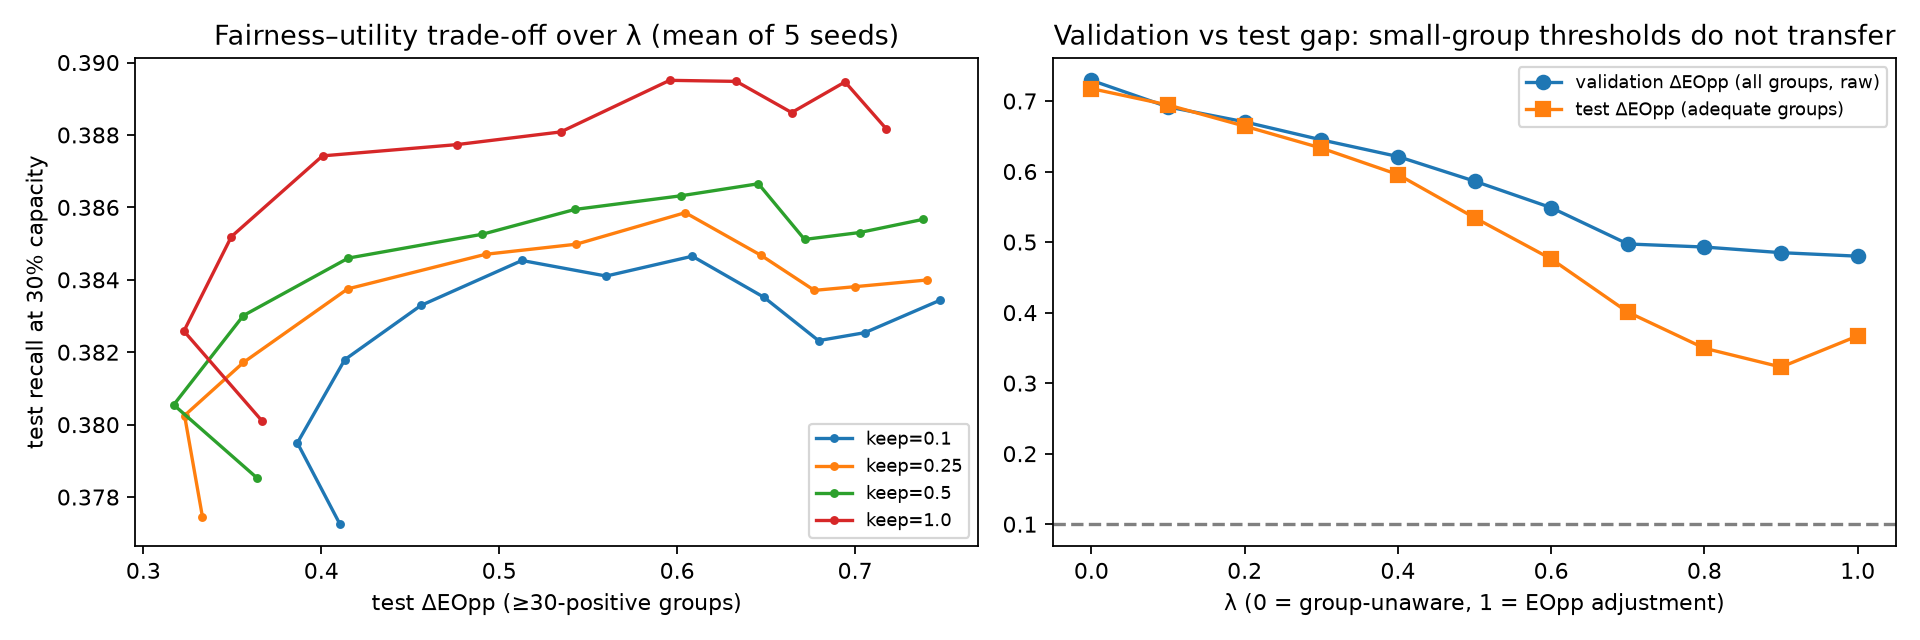
\includegraphics[width=0.9\textwidth]{tradeoff_curves.png}
\caption{Fairness--utility trade-off over $\lambda$ and validation vs test gaps (mean of 5 splits).}\label{fig:tradeoff}
\end{figure}

\subsection{Audit procedure: simulation evidence (SYNTHETIC and SEMI-SYNTHETIC)}
\begin{table}[h]\centering\small
\caption{SYNTHETIC (\sect{8}): 16 groups of 4000 to 8 positives, one 20-positive group 0.20 below the rest, $R=300$, $\epsilon=0.10$.}\label{tab:sim}
% generated by make_tables.py from ../results; do not edit by hand
\begin{tabular}{lcccccc}
\toprule
& \multicolumn{3}{c}{FTS (exceptional group kept)} & ACC & \multicolumn{2}{c}{90\% gap interval} \\
\cmidrule(lr){2-4}\cmidrule(lr){6-7}
Estimator $\cdot$ rule & 100\% & 50\% & 25\% & homog. & coverage & width \\
\midrule
raw $\cdot$ plugin & 0.003 & 0.000 & 0.000 & 0.007 & -- & -- \\
independent $\cdot$ upper 0.9 & 0.000 & 0.000 & 0.000 & 0.000 & 0.264 & 0.382 \\
complete $\cdot$ plugin & 1.000 & 1.000 & 1.000 & 1.000 & 0.000 & 0.000 \\
hier $\cdot$ plugin & 1.000 & 1.000 & 1.000 & 1.000 & 0.000 & 0.018 \\
hier $\cdot$ upper 0.9 & 0.980 & 0.987 & 0.987 & 0.993 & 0.000 & 0.018 \\
fullbayes $\cdot$ plugin & 0.983 & 1.000 & 0.993 & 1.000 & 0.038 & 0.114 \\
fullbayes $\cdot$ upper 0.9 & 0.310 & 0.337 & 0.397 & 0.427 & 0.038 & 0.114 \\
\textbf{proposed $\pi\le$0.8 $\cdot$ plugin (calibrated)} & 0.503 & 0.593 & 0.563 & 0.830 & 0.962 & 0.399 \\
proposed $\pi\le$0.8 $\cdot$ upper 0.5 & 0.450 & 0.567 & 0.577 & 0.773 & 0.962 & 0.399 \\
proposed $\pi\le$0.8 $\cdot$ upper 0.9 & 0.000 & 0.000 & 0.000 & 0.000 & 0.962 & 0.399 \\
proposed $\pi\le$0.95 $\cdot$ upper 0.9 & 0.297 & 0.300 & 0.317 & 0.527 & 0.589 & 0.273 \\
proposed $\pi\le$0.99 $\cdot$ upper 0.9 & 0.780 & 0.830 & 0.883 & 0.930 & 0.200 & 0.114 \\
\bottomrule
\end{tabular}

\end{table}

\begin{table}[h]\centering\small
\caption{SEMI-SYNTHETIC (\sect{9.2}): the real seed-0 validation design (32 groups, 1 to 5,499 positives), invented TPRs.
The deficit is at \texttt{2|2|1} (Black, female, disabled; 24 positives), thinned to 25\% in the ``keep .25'' columns. $R=300$.}\label{tab:semi}
\resizebox{\textwidth}{!}{% generated by make_tables.py from ../results; do not edit by hand
\begin{tabular}{lcccccccc}
\toprule
& ACC & \multicolumn{2}{c}{FTS cell} & \multicolumn{2}{c}{FTS interaction} & FTS dis. & \multicolumn{2}{c}{$\theta_{2|2|1}$ (cell, keep 1)} \\
\cmidrule(lr){3-4}\cmidrule(lr){5-6}\cmidrule(lr){8-9}
Procedure & keep 1 & keep 1 & keep .25 & keep 1 & keep .25 & keep 1 & 90\% cov. & post. mean \\
\midrule
\textbf{proposed (robust@0.8, plugin)} & 0.323 & 0.133 & 0.280 & 0.160 & 0.233 & 0.000 & 0.720 & 0.281 \\
fullbayes $\cdot$ plugin & 0.997 & 1.000 & 0.997 & 1.000 & 1.000 & 0.000 & 0.000 & 0.371 \\
fullbayes $\cdot$ upper0.9 & 0.413 & 0.397 & 0.477 & 0.520 & 0.540 & 0.000 & 0.000 & 0.371 \\
hier $\cdot$ plugin & 1.000 & 1.000 & 0.997 & 1.000 & 1.000 & 0.000 & 0.000 & 0.378 \\
hier $\cdot$ upper0.9 & 0.970 & 0.997 & 0.983 & 0.993 & 0.987 & 0.000 & 0.000 & 0.378 \\
independent $\cdot$ plugin & 0.000 & 0.000 & 0.000 & 0.000 & 0.000 & 0.000 & 0.900 & 0.201 \\
independent $\cdot$ upper0.9 & 0.000 & 0.000 & 0.000 & 0.000 & 0.000 & 0.000 & 0.900 & 0.201 \\
raw $\cdot$ plugin & 0.000 & 0.000 & 0.000 & 0.000 & 0.000 & 0.000 & -- & -- \\
struct $\cdot$ plugin & 0.277 & 0.293 & 0.367 & 0.367 & 0.363 & 0.000 & 0.000 & 0.368 \\
struct $\cdot$ upper0.9 & 0.217 & 0.233 & 0.327 & 0.320 & 0.313 & 0.000 & 0.000 & 0.368 \\
\bottomrule
\end{tabular}
}
\end{table}

The calibrated procedure has FTS 0.503 and ACC 0.830 on the synthetic calibration design. On the real design its FTS is
0.133--0.280, but \textbf{its ACC drops to 0.32}. The calibration is design-specific and must be redone on the deployment
design. Exchangeable pooling (hier) declares the 24-positive exception ``fair'' in 98--100\% of worlds, and the
attribute-structured audit masks it whenever the deficit is an interaction. Every estimator detects a deficit carried by
the disability main effect.

\begin{figure}[h]\centering
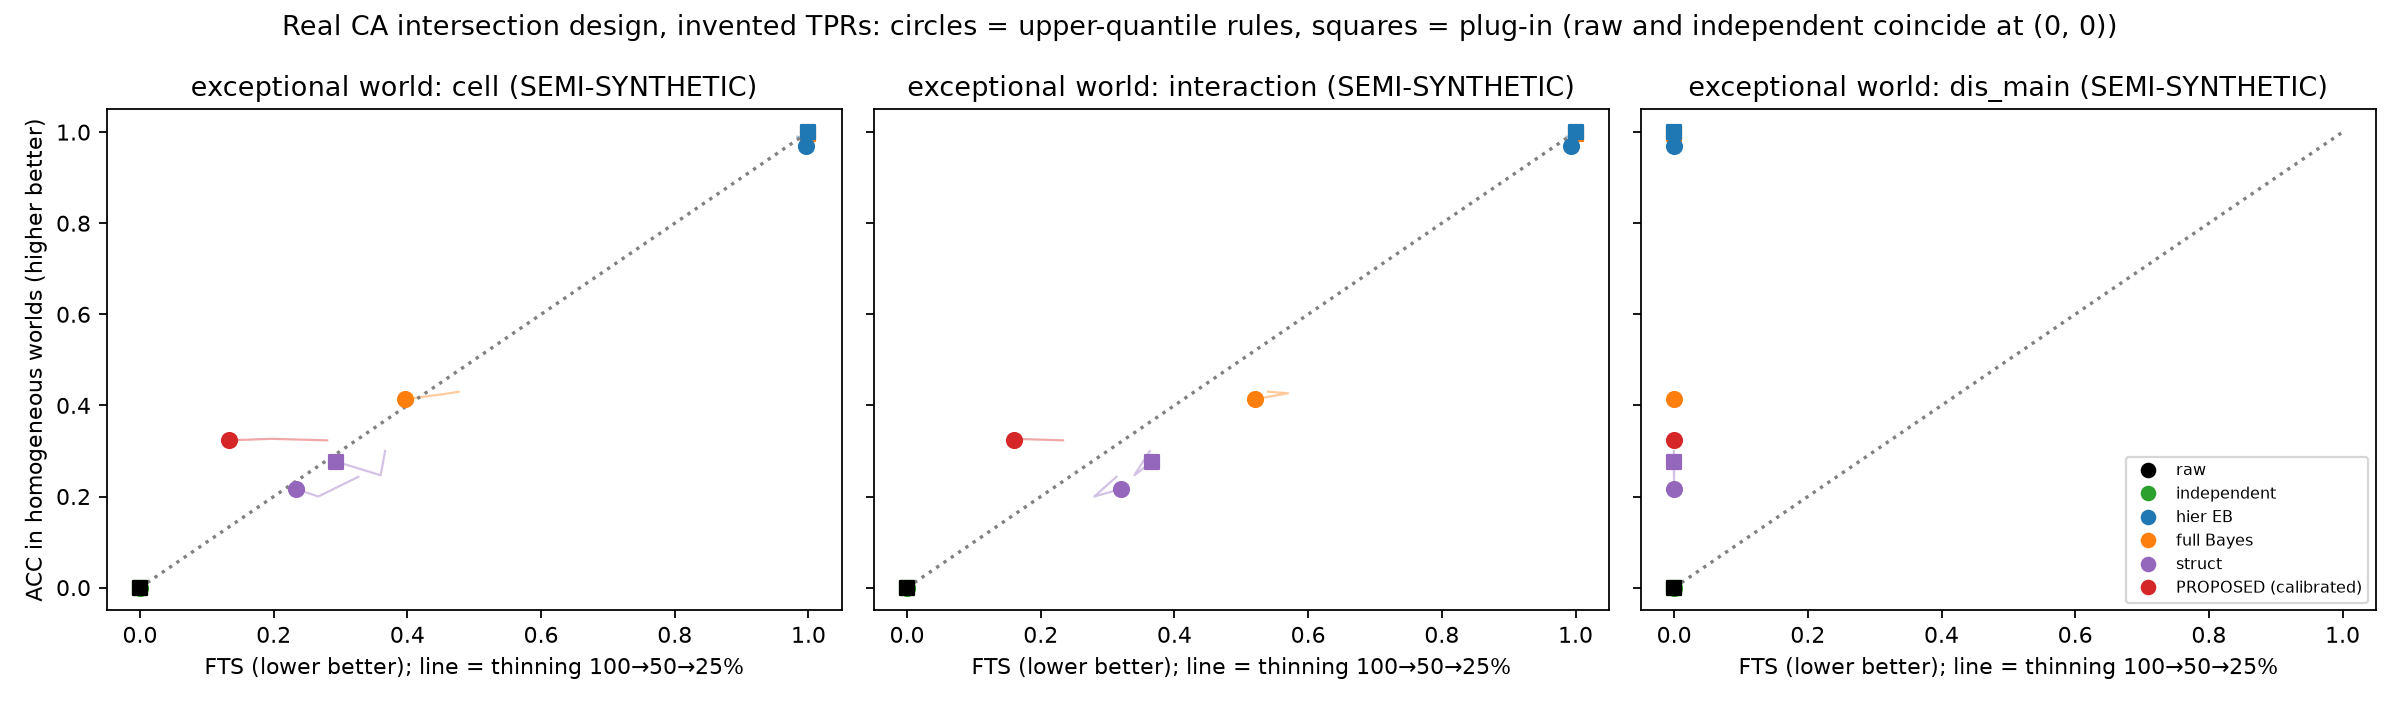
\includegraphics[width=\textwidth]{semisynthetic_frontier.png}
\caption{SEMI-SYNTHETIC tolerance-decision frontier on the real CA design.}\label{fig:semi}
\end{figure}

\subsection{Improved procedure: design-matched calibration and held-out certification (\sect{15})}
Preregistered hypotheses H2a--c were tested out of sample on the Texas design (Table~\ref{tab:v2}, Figure~\ref{fig:v2}).
The design-matched audit scores $J=\text{ACC}-\text{mean FTS}=0.664$, against at most 0.385 for every established audit
and 0.189 for the invented-design calibration. Its false-certification rate is 0.168, against 0.615--0.661 for
hierarchical and full-Bayes pooling (H2a, H2b supported). On the California design, which the pilot used, it only ties
the pooled audits on $J$ (0.330 vs 0.333--0.334), with half their false-certification rate. Held-out certification made no
false tolerance claims on real CA or TX data, against 10 of 10 false claims with same-data certification, at unchanged
recall (Table~\ref{tab:v2real}; H2c supported).

\begin{table}[h]\centering\small
\caption{Out-of-sample test on the Texas design (SEMI-SYNTHETIC; $R=200$ per cell).}\label{tab:v2}
\resizebox{\textwidth}{!}{% generated by make_tables.py from ../results; do not edit by hand
\begin{tabular}{lccccccc}
\toprule
& ACC & \multicolumn{3}{c}{FTS} & mean & & 90\% gap \\
\cmidrule(lr){3-5}
Procedure & (fair) & cell & interaction & dis.\ main & FTS & $J$ & coverage \\
\midrule
\textbf{design-matched (centred-slab contam., $\pi{\le}$0.95 $\cdot$ upper 0.5)} & 0.832 & 0.255 & 0.250 & 0.000 & 0.168 & \textbf{0.664} & 0.615 \\
fullbayes $\cdot$ plugin & 1.000 & 0.920 & 0.925 & 0.000 & 0.615 & \textbf{0.385} & 0.174 \\
hier $\cdot$ upper 0.9 & 0.985 & 0.930 & 0.945 & 0.000 & 0.625 & \textbf{0.360} & 0.013 \\
hier $\cdot$ plugin & 1.000 & 0.990 & 0.992 & 0.000 & 0.661 & \textbf{0.339} & 0.013 \\
fullbayes $\cdot$ upper 0.9 & 0.290 & 0.110 & 0.145 & 0.000 & 0.085 & \textbf{0.205} & 0.174 \\
\S9 procedure (contam., $\pi{\le}$0.8 $\cdot$ plugin) & 0.218 & 0.048 & 0.038 & 0.000 & 0.028 & \textbf{0.189} & 0.506 \\
struct $\cdot$ plugin & 0.108 & 0.125 & 0.095 & 0.000 & 0.073 & \textbf{0.034} & 0.037 \\
struct $\cdot$ upper 0.9 & 0.090 & 0.105 & 0.078 & 0.000 & 0.061 & \textbf{0.029} & 0.037 \\
independent $\cdot$ upper 0.9 & 0.000 & 0.000 & 0.000 & 0.000 & 0.000 & \textbf{0.000} & 0.000 \\
raw $\cdot$ plugin & 0.000 & 0.000 & 0.000 & 0.000 & 0.000 & \textbf{0.000} & -- \\
\bottomrule
\end{tabular}
}
\end{table}
\begin{figure}[h]\centering
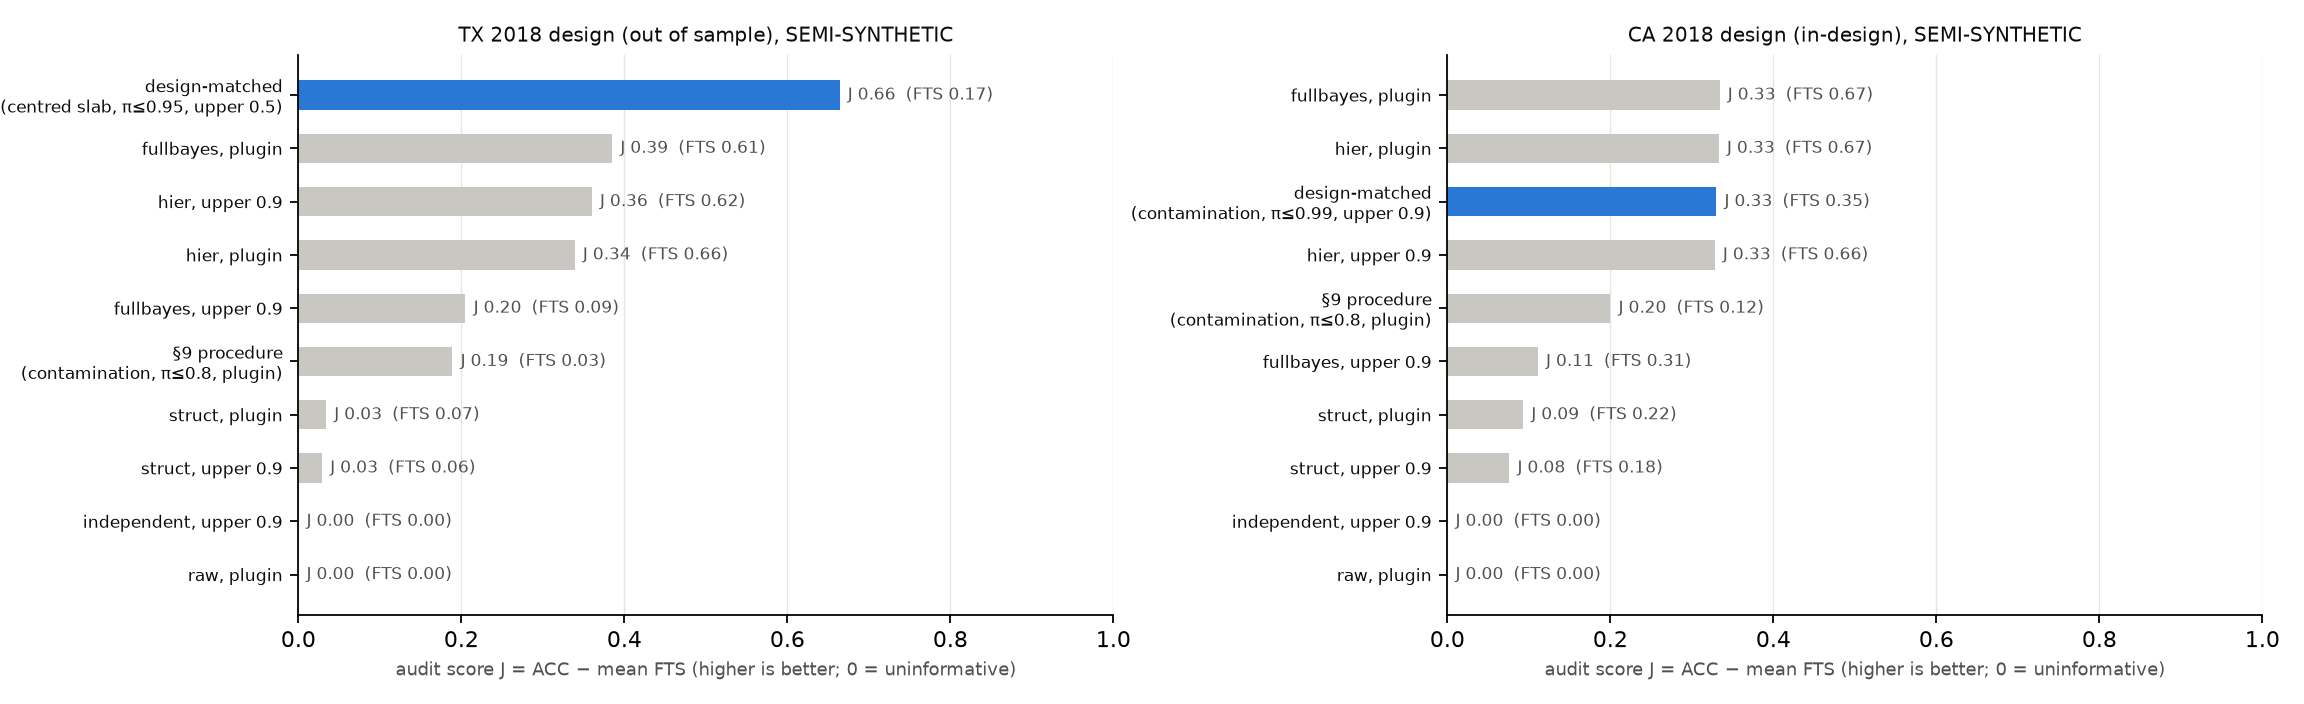
\includegraphics[width=\textwidth]{v2_audit_score.png}
\caption{Audit score $J$ per procedure on the Texas (out of sample) and California designs.}\label{fig:v2}
\end{figure}
\begin{table}[h]\centering\small
\caption{Real data: tolerance claims of the design-matched procedure, same-data vs held-out certification.}\label{tab:v2real}
% generated by make_tables.py from ../results; do not edit by hand
\begin{tabular}{llcccc}
\toprule
State & certification & claims ($\le\epsilon$) & false claims & mean test $\Delta$EOpp & mean test recall \\
\midrule
CA & same-data & 5/5 & 5 & 0.367 & 0.380 \\
CA & held-out & 0/5 & 0 & 0.351 & 0.379 \\
TX & same-data & 5/5 & 5 & 0.238 & 0.350 \\
TX & held-out & 0/5 & 0 & 0.267 & 0.350 \\
\bottomrule
\end{tabular}

\end{table}

\section{Ethical considerations}
\begin{itemize}
  \item \textbf{Systematic exclusion of disabled people:} the unconstrained rule almost never selects disabled people
    without public coverage. Any real outreach built this way would miss them.
  \item \textbf{Pooling can erase small groups:} a hierarchical audit can report a small disadvantaged intersection as
    average. Report raw counts and the pooling pull next to every pooled estimate.
  \item \textbf{Who chooses $\epsilon$ and the capacity:} the analysts chose $\epsilon=\epsTol{}$ and \capacity{}
    capacity; they were not set by affected communities. No stakeholder input was obtained: no affected community, outreach agency or disability organisation was consulted on $\epsilon$, the capacity or the label. This is a limitation, and both values are reported with sensitivity analyses ($\epsilon\in\{0.05,0.10,0.15\}$).
  \item \textbf{Label meaning:} absence of public coverage is not uninsurance (people may hold private coverage) and is not
    eligibility. Mislabelling these concepts could misdirect resources.
  \item \textbf{Recorded categories:} race and disability categories are survey constructs. Keeping all nine race codes
    preserves their meaning but creates very small cells.
\end{itemize}

\section{Caveats and recommendations}\label{sec:caveats}
\begin{itemize}
  \item No rule in the family reaches $\Delta$EOpp $\le0.10$ on test; the smallest observed value is 0.227.
    \textbf{Do not describe any configuration as fair.}
  \item Do not certify a tolerance from a pooled estimate when any intersection has fewer than about 30 positives.
    Validation-time claims did not transfer to test.
  \item Bayesian credible intervals are not frequentist guarantees. The EB struct audit covers 0.665 at nominal 0.90 even
    under its own model (oracle 0.905), and exchangeable pooling gives near-zero coverage for the gap in simulation.
  \item Calibrate the audit procedure on the design it will be used on, and certify on data not used to choose the rule.
    The invented-design calibration lost acceptance (ACC 0.83 $\to$ 0.32), while design-matched calibration reached
    $J=0.664$ out of sample; same-data certification produced 10 of 10 false claims, held-out certification none.
  \item Results are for the unweighted benchmark sample unless stated. The survey-weighted estimates cover the
    sex$\times$disability groups only.
  \item \textbf{Relation to prior work.} Hierarchical Bayesian estimation of intersectional fairness is not ours (Foulds et al.\ 2020); our \texttt{struct} audit is a restricted version in that spirit, not an exact reproduction. That marginal fairness can hide subgroup unfairness is known (Kearns et al.\ 2018); our interaction-only world is an instance. That fairness constraints met on training data can fail out of sample is known (Cotter et al.\ 2019). Our contribution is the evaluation of pooled \emph{audit criteria} under sparsity and the design-matched, held-out audit protocol, not a new prior or metric.
\end{itemize}

\clearpage
\begin{landscape}
\appendix
\section{Intersectional audit table}
{\small\setlength{\tabcolsep}{4pt}% generated by make_tables.py from ../results; do not edit by hand
\begin{longtable}{lllcrrrcccccc}
\caption{Intersectional audit table for the BN rule (unconstrained top-30\%, seed-0 test split). $n$ = people, $n^+$ = positives (no public coverage), $k$ = selected positives, TPR = $k/n^+$. Posterior means under each audit model; pull = hier $-$ raw. The contamination column uses $\pi_{\max}=0.95$ because this table is computed (notebook \S7) before the \S9 calibration fixes $\pi_{\max}=0.8$. $\ast$ = exploratory ($<30$ positives or $<30$ negatives).}\label{tab:groups}\\
\toprule
Code & Race (RAC1P) & Sex & Disab. & $n$ & $n^+$ & $k$ & raw TPR & indep. & hier & struct & contam.\,$\pi{\le}0.95$ & pull \\
\midrule
\endfirsthead
\toprule
Code & Race (RAC1P) & Sex & Disab. & $n$ & $n^+$ & $k$ & raw TPR & indep. & hier & struct & contam.\,$\pi{\le}0.95$ & pull \\
\midrule
\endhead
\texttt{7|2|1} & NHPI & F & yes & 4 & 0 & 0 & -- & -- & -- & -- & -- & --\textcolor{red!70!black}{$\ast$} \\
\texttt{4|2|2} & Alaska Native & F & no & 1 & 1 & 0 & 0.000 & 0.324 & 0.129 & 0.000 & 0.137 & 0.129\textcolor{red!70!black}{$\ast$} \\
\texttt{4|2|1} & Alaska Native & F & yes & 2 & 1 & 0 & 0.000 & 0.330 & 0.130 & 0.000 & 0.130 & 0.130\textcolor{red!70!black}{$\ast$} \\
\texttt{4|1|1} & Alaska Native & M & yes & 1 & 1 & 0 & 0.000 & 0.337 & 0.132 & 0.000 & 0.127 & 0.132\textcolor{red!70!black}{$\ast$} \\
\texttt{5|2|1} & AIAN, tribe spec./n.s. & F & yes & 9 & 2 & 0 & 0.000 & 0.248 & 0.105 & 0.006 & 0.104 & 0.105\textcolor{red!70!black}{$\ast$} \\
\texttt{7|1|1} & NHPI & M & yes & 8 & 2 & 0 & 0.000 & 0.252 & 0.103 & 0.033 & 0.105 & 0.103\textcolor{red!70!black}{$\ast$} \\
\texttt{3|2|1} & American Indian & F & yes & 16 & 3 & 0 & 0.000 & 0.197 & 0.085 & 0.005 & 0.080 & 0.085\textcolor{red!70!black}{$\ast$} \\
\texttt{5|1|1} & AIAN, tribe spec./n.s. & M & yes & 14 & 6 & 0 & 0.000 & 0.124 & 0.055 & 0.003 & 0.053 & 0.055\textcolor{red!70!black}{$\ast$} \\
\texttt{3|1|1} & American Indian & M & yes & 20 & 7 & 0 & 0.000 & 0.110 & 0.050 & 0.003 & 0.049 & 0.050\textcolor{red!70!black}{$\ast$} \\
\texttt{5|1|2} & AIAN, tribe spec./n.s. & M & no & 24 & 14 & 1 & 0.071 & 0.127 & 0.088 & 0.100 & 0.088 & 0.017\textcolor{red!70!black}{$\ast$} \\
\texttt{2|2|1} & Black & F & yes & 142 & 21 & 0 & 0.000 & 0.044 & 0.019 & 0.003 & 0.019 & 0.019\textcolor{red!70!black}{$\ast$} \\
\texttt{5|2|2} & AIAN, tribe spec./n.s. & F & no & 37 & 25 & 5 & 0.200 & 0.221 & 0.199 & 0.183 & 0.199 & $-$0.001\textcolor{red!70!black}{$\ast$} \\
\texttt{2|1|1} & Black & M & yes & 187 & 26 & 0 & 0.000 & 0.036 & 0.017 & 0.002 & 0.017 & 0.017\textcolor{red!70!black}{$\ast$} \\
\texttt{9|2|1} & Two or more & F & yes & 77 & 29 & 1 & 0.034 & 0.064 & 0.047 & 0.030 & 0.047 & 0.013\textcolor{red!70!black}{$\ast$} \\
\texttt{9|1|1} & Two or more & M & yes & 97 & 32 & 0 & 0.000 & 0.030 & 0.013 & 0.015 & 0.013 & 0.013 \\
\texttt{7|1|2} & NHPI & M & no & 48 & 32 & 17 & 0.531 & 0.528 & 0.506 & 0.554 & 0.506 & $-$0.025\textcolor{red!70!black}{$\ast$} \\
\texttt{6|1|1} & Asian & M & yes & 125 & 34 & 1 & 0.029 & 0.056 & 0.040 & 0.040 & 0.041 & 0.011 \\
\texttt{7|2|2} & NHPI & F & no & 57 & 38 & 28 & 0.737 & 0.725 & 0.704 & 0.716 & 0.705 & $-$0.032\textcolor{red!70!black}{$\ast$} \\
\texttt{3|1|2} & American Indian & M & no & 84 & 44 & 3 & 0.068 & 0.088 & 0.074 & 0.089 & 0.075 & 0.006 \\
\texttt{8|1|1} & Some other race & M & yes & 209 & 49 & 0 & 0.000 & 0.019 & 0.009 & 0.002 & 0.009 & 0.009 \\
\texttt{3|2|2} & American Indian & F & no & 89 & 55 & 10 & 0.182 & 0.192 & 0.183 & 0.165 & 0.183 & 0.002 \\
\texttt{8|2|1} & Some other race & F & yes & 197 & 56 & 1 & 0.018 & 0.035 & 0.025 & 0.005 & 0.024 & 0.007 \\
\texttt{6|2|1} & Asian & F & yes & 159 & 64 & 5 & 0.078 & 0.091 & 0.083 & 0.077 & 0.082 & 0.005 \\
\texttt{1|1|1} & White & M & yes & 965 & 289 & 3 & 0.010 & 0.014 & 0.012 & 0.012 & 0.012 & 0.002 \\
\texttt{2|2|2} & Black & F & no & 541 & 312 & 31 & 0.099 & 0.102 & 0.100 & 0.114 & 0.100 & 0.001 \\
\texttt{1|2|1} & White & F & yes & 1046 & 365 & 10 & 0.027 & 0.030 & 0.028 & 0.025 & 0.028 & 0.001 \\
\texttt{2|1|2} & Black & M & no & 655 & 377 & 27 & 0.072 & 0.074 & 0.073 & 0.060 & 0.072 & 0.001 \\
\texttt{9|1|2} & Two or more & M & no & 547 & 384 & 149 & 0.388 & 0.389 & 0.387 & 0.362 & 0.386 & $-$0.001 \\
\texttt{9|2|2} & Two or more & F & no & 643 & 450 & 231 & 0.513 & 0.513 & 0.512 & 0.534 & 0.511 & $-$0.001 \\
\texttt{6|1|2} & Asian & M & no & 1488 & 1030 & 634 & 0.616 & 0.615 & 0.615 & 0.602 & 0.614 & 0.000 \\
\texttt{8|1|2} & Some other race & M & no & 1824 & 1139 & 100 & 0.088 & 0.088 & 0.088 & 0.084 & 0.088 & 0.000 \\
\texttt{8|2|2} & Some other race & F & no & 2273 & 1320 & 201 & 0.152 & 0.153 & 0.152 & 0.156 & 0.152 & 0.000 \\
\texttt{6|2|2} & Asian & F & no & 2283 & 1727 & 1288 & 0.746 & 0.745 & 0.745 & 0.753 & 0.745 & $-$0.001 \\
\texttt{1|1|2} & White & M & no & 5805 & 3980 & 1233 & 0.310 & 0.310 & 0.310 & 0.317 & 0.310 & 0.000 \\
\texttt{1|2|2} & White & F & no & 7976 & 5570 & 2734 & 0.491 & 0.491 & 0.491 & 0.486 & 0.491 & 0.000 \\
\bottomrule
\end{longtable}
}
\section{Confirmatory and exploratory paired bootstrap (seed 0, $B=1000$)}\label{tab:conf}
{\small% generated by make_tables.py from ../results; do not edit by hand
\begin{tabular}{llcrccc}
\toprule
Comparison & family & metric & estimate & 95\% CI & $p_{\text{boot}}$ & $p_{\text{Holm}}$ \\
\midrule
calibrated $-$ hier plug-in & confirmatory & $\Delta$EOpp & $+0.0000$ & $[+0.0000, +0.0000]$ & 1.000 & 1.000 \\
calibrated $-$ hier plug-in & confirmatory & recall & $+0.0000$ & $[+0.0000, +0.0000]$ & 1.000 & -- \\
calibrated $-$ raw plug-in & confirmatory & $\Delta$EOpp & $-0.0517$ & $[-0.1944, +0.0505]$ & 0.368 & 0.736 \\
calibrated $-$ raw plug-in & confirmatory & recall & $-0.0061$ & $[-0.0089, -0.0035]$ & 0.001 & -- \\
proposed upper $-$ hier plug-in & exploratory & $\Delta$EOpp & $-0.0714$ & $[-0.1755, +0.0000]$ & 0.074 & -- \\
proposed upper $-$ hier plug-in & exploratory & recall & $-0.0026$ & $[-0.0048, -0.0005]$ & 0.014 & -- \\
proposed upper $-$ raw plug-in & exploratory & $\Delta$EOpp & $-0.1231$ & $[-0.3073, +0.0091]$ & 0.076 & -- \\
proposed upper $-$ raw plug-in & exploratory & recall & $-0.0086$ & $[-0.0124, -0.0053]$ & 0.001 & -- \\
struct upper $-$ hier plug-in & exploratory & $\Delta$EOpp & $-0.0714$ & $[-0.1755, +0.0000]$ & 0.074 & -- \\
struct upper $-$ hier plug-in & exploratory & recall & $-0.0026$ & $[-0.0048, -0.0005]$ & 0.014 & -- \\
struct upper $-$ raw plug-in & exploratory & $\Delta$EOpp & $-0.1231$ & $[-0.3073, +0.0091]$ & 0.076 & -- \\
struct upper $-$ raw plug-in & exploratory & recall & $-0.0086$ & $[-0.0124, -0.0053]$ & 0.001 & -- \\
struct plug-in $-$ hier plug-in & exploratory & $\Delta$EOpp & $-0.0714$ & $[-0.1755, +0.0000]$ & 0.074 & -- \\
struct plug-in $-$ hier plug-in & exploratory & recall & $-0.0026$ & $[-0.0048, -0.0005]$ & 0.014 & -- \\
struct plug-in $-$ raw plug-in & exploratory & $\Delta$EOpp & $-0.1231$ & $[-0.3073, +0.0091]$ & 0.076 & -- \\
struct plug-in $-$ raw plug-in & exploratory & recall & $-0.0086$ & $[-0.0124, -0.0053]$ & 0.001 & -- \\
\bottomrule
\end{tabular}
}

\medskip\noindent The confirmatory family (Holm) is the calibrated procedure vs hier plug-in and vs raw plug-in, on test
$\Delta$EOpp. All other rows are exploratory. Training uncertainty (5 refits): calibrated $-$ raw plug-in
$=-0.016\pm0.039$ (signs $-+-0-$); calibrated $-$ hier plug-in $=+0.009\pm0.035$ (signs $0++-0$).
\end{landscape}
\end{document}
